\section{Experiments}
\begin{table}[t]
  \centering
  \vspace{8pt}
  \tabcolsep=0.11cm{
  \begin{tabular}{ccccc}
    \toprule[1.5pt]
      \textbf{\# Objects} & \textbf{System} & \textbf{\% Solved (SD)} & \textbf{Avg Ref Time (s)} & \textbf{Avg \# MP Calls}\\
    \midrule[2pt]
      30 (can) & T & 42 (0) & 6.2 & 8.0\\
    \midrule
      30 (can) & B & 40 (0) & 20.5 & 10.5\\
    \midrule
      30 (can) & L & 72 (8.2) & 20.4 & 11.3\\
    \midrule
      30 (can) & F & 81 (3.0) & 17.9 & 12.7\\
    \midrule[1.5pt]
      35 (can) & T & 50 (0) & 9.2 & 8.0\\
    \midrule
      35 (can) & B & 50 (0) & 17.6 & 9.2\\
    \midrule
      35 (can) & L & 68 (8.3) & 11.6 & 6.6\\
    \midrule
      35 (can) & F & 78 (2.2) & 10.6 & 6.8\\
    \midrule[1.5pt]
      40 (can) & T & 34 (0) & 19.7 & 10.3\\
    \midrule
      40 (can) & B & 36 (0) & 21.7 & 10.0\\
    \midrule
      40 (can) & L & 61 (6.3) & 18.7 & 9.4\\
    \midrule
      40 (can) & F & 74 (3.2) & 20.7 & 10.4\\
    \midrule[2pt]
    %   2 (dinner) & T & 100 (0) & 35.5 & 60.2\\
    % \midrule
    %   2 (dinner) & B & 100 (0) & 37.3 & 59.2\\
    % \midrule
    %   2 (dinner) & L & 99 (1.8) & 41.5 & 61.6\\
    % \midrule[1.5pt]
      4 (dinner) & T & 100 (0) & 43.2 & 98.0\\
    \midrule
      4 (dinner) & B & 90 (0) & 63.0 & 95.5\\
    \midrule
      4 (dinner) & L & 99 (0.6) & 69.2 & 97.1\\
    \midrule[2pt]
      2 (frying) & T & 96 (0) & 29.0 & 67.2\\
    \midrule
      2 (frying) & B & 88 (0) & 46.9 & 60.0\\
    \midrule
      2 (frying) & L & 99 (2.0) & 22.6 & 44.7\\
    \midrule[1.5pt]
      4 (frying) & T & 55 (0) & 48.9 & 131.8\\
    \midrule
      4 (frying) & B & 20 (0) & 187.9 & 155.5\\
    \midrule
      4 (frying) & L & 92 (6.8) & 90.6 & 120.9\\
    \bottomrule[1.5pt]
  \end{tabular}}
  \caption{\small{Percent solved, standard deviation, and average refinement time \& number of motion
      planning calls on successes, for baseline 1 (T); baseline 2
      (B); learned refinement policies with greedy graph search (L);
      and our full system: learned refinement policies and graph
      search heuristics (F). L and F results are averaged across 5
      separately trained sets of weights. Time limit: 300s.}}
  \label{table:results}
\end{table}

\subsection{Methodology}
We evaluate our approach in three domains: cans distributed randomly
on a table (the \emph{can domain}), setting up bowls for dinner (the
\emph{dinner domain}), and placing frying pans into a narrow shelf
(the \emph{frying domain}).  We compare performance with two
baselines, both of which use the hand-coded refinement distributions
used in {\sc sfrcra-14}.

Baseline 1 is {\sc sfrcra-14}: it uses exhaustive backtracking search
for refinement and greedy depth-first search of the {\sc prg}, which
always tries to refine the plan that incorporates all error
information obtained thus far.  Baseline 2 uses randomized refinement
with the following fixed graph search policy: try 3 times to refine
the deepest node in the graph; if unsuccessful, generate a geometric
error, replan with the task planner (which creates a child node), and
repeat.

We compare these baselines against two systems. The first combines
learned refinement policies with the graph search used in baseline
2. The second is our full system, and uses learned refinement policies
and graph search heuristics.  For the dinner domain and frying domain,
we focus only on the low-level learning. Since the errors propagated in these
domains only relate to the stackability of objects, a good graph search strategy
incorporates all available error information when
attempting refinement. Thus, the graph search strategy from baseline 2
already performs well.

Initial experimentation revealed that jointly learning weights for all
parameter types was intractable. Thus, we use a curriculum where the
distribution of planning problems, $\Prob$, gets progressively
harder. For the full system, we train the refinement policies first,
then fix them while collecting demonstrations and training the graph
search heuristics. To reduce variance in the process, we train 3 sets
of refinement weights independently and select the one that performs
best on a validation set.

We report results on fixed test sets of 50 randomly generated
environments for the can and dinner domains, and 20 for the frying
domain (because these environments have less variation).  For the
third and fourth systems, we average results across running the
training process 5 times independently and evaluating each final set
of weights.

Our low-level policies use 24 features and rely on the notion of a
target object. 9 binary features encode the bucketed distance between
the sample and target object. 9 binary features encode the bucketed
sample height. 3 features describe the number of other objects within
discs of radius 7, 10, and 15 centimeters around the sample. 3 binary
features describe the angle made between the vector from the robot to
the target and the vector from the sample to the target: whether the
angle is less than $\pi/3$, $\pi/2$, and $3\pi/4$.

Our high-level heuristics use features to describe the feasibility of
plans. In our domains, this mainly summarizes issues with potential
grasps. We use three features to evaluate a potential grasp action,
targeted at an object $o$. We consider a cone whose point is at the
object center and ranges from angles $-\frac{\pi}{3}$ to
$\frac{\pi}{3}$, pointing toward the closest table edge from $o$. The
exists\_obstr feature is a binary variable that indicates whether any
other objects lie in this cone. The exists\_path feature is a binary
variable that indicates whether there is a linear grasp path wide
enough for the robot's gripper to fit through within the cone. The
sweep\_count feature computes the minimum number of collisions with the robot's
gripper placed at any angle inside the cone.

We construct these features for the first five grasp actions in the
plan, padding with -1 as necessary. We then add on the following
aggregate features associated with the entire plan: 1) the minimum
exists\_obstr across all grasp actions, 2) the sum of sweep\_count
across all grasp actions, 3) the number of times $u$ was picked for
refinement, and 4) the number of times $u$ was picked for generating
an error.

Our experiments are conducted in Python 2.7 using the OpenRave
simulator~\cite{Diankov_2008_6117} with a PR2 robot.  The motion
planner we use is trajopt~\cite{schulman2013finding}, and the task
planner is Fast-Forward~\cite{FF}.  The experiments were carried out
in series on an Intel Core i7-4770K machine with 16GB RAM. The time limit
for each problem was 300 seconds. Table
\ref{table:results} summarizes our quantitative results.

% \begin{figure}[t]
%   \centering
%   \begin{subfigure}[b]{0.35\linewidth}
%     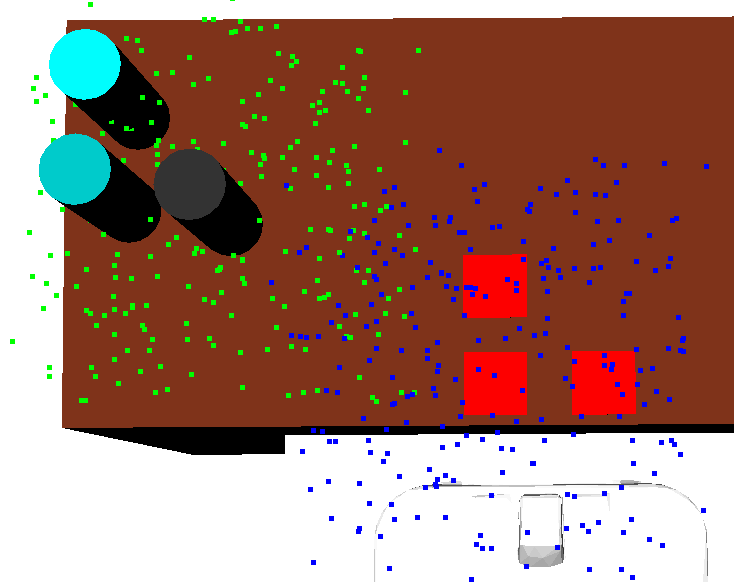
\includegraphics[width=\textwidth]{images/learns.png}
%     \caption{Initial distributions.}
%   \end{subfigure}
%   \begin{subfigure}[b]{0.35\linewidth}
%     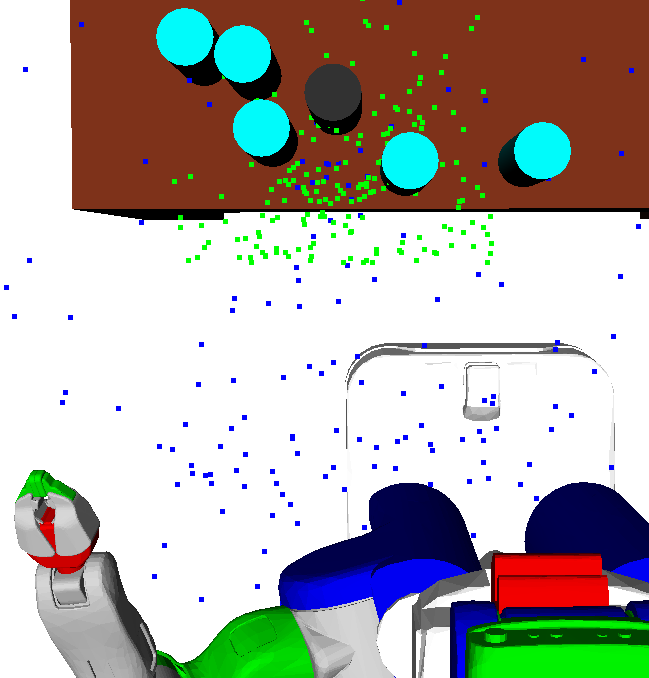
\includegraphics[width=\textwidth]{images/learn4.png}
%     \caption{After 4 iterations.}
%   \end{subfigure}
%   \begin{subfigure}[b]{0.35\linewidth}
%     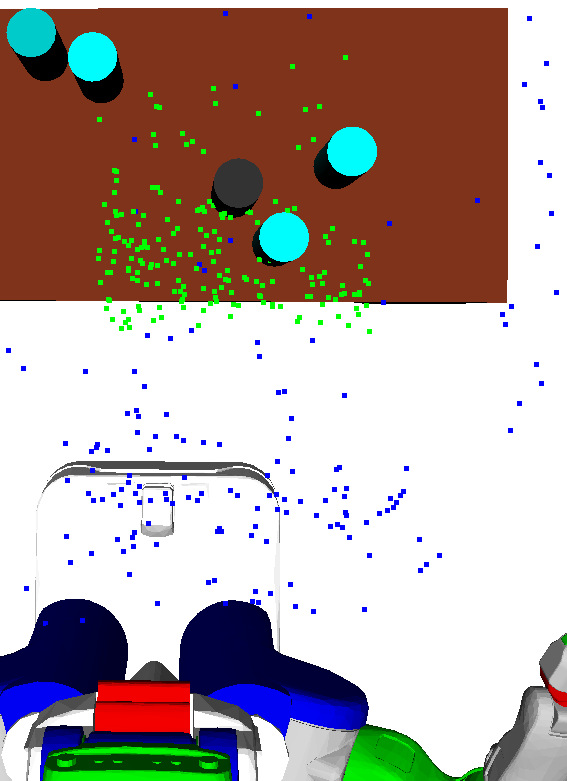
\includegraphics[width=\textwidth]{images/learn8.png}
%     \caption{After 8 iterations.}
%   \end{subfigure}
%   \begin{subfigure}[b]{0.35\linewidth}
%     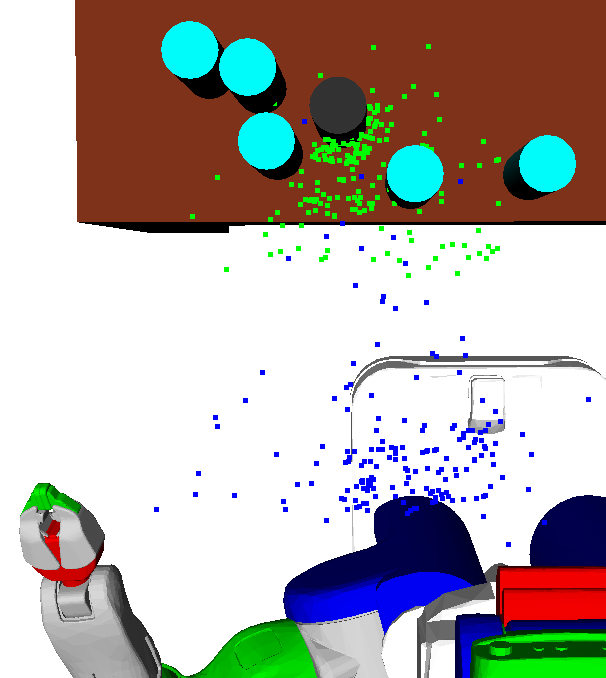
\includegraphics[width=\textwidth]{images/learn12.png}
%     \caption{Final distributions.}
%   \end{subfigure}
%   \caption{\small{Learned base position (blue) and left arm grasp (green) distributions used to
% pick up the black can after different training iterations for learning refinement policies.
% An iteration refers to a single planning problem,
% which terminates after $H$ calls to the \textsc{Resample} routine.
% Initial distributions are uniform because we initialize weights to $\vec{\mathbf{0}}$.
% Final distributions are after 12 iterations.}}
%   \label{fig:training}
% \end{figure}

\subsection{Can Domain}
We run three sets of experiments, using 30, 35, and 40 cans on the
table.  The goal is always for the robot to pick up a particular can
with its left gripper. We disable the right gripper, so any
obstructions to the target object must be picked up and placed
elsewhere on the table. This domain has 4 types of continuous
references: base poses, object grasping poses, object putdown poses,
and object putdown locations.

Our curriculum learning system trains distributions for base poses and
grasping poses for 12 iterations with $\epsilon = 5$, then base poses,
grasping poses, and putdown poses (at fixed location) for 18
iterations with $\epsilon = 20$, then all reference types for 30
iterations with $\epsilon = 20$. We fix $H = 100$.

To train the graph search heuristics, we collected approximately 300
optimal actions from the human demonstrator, over 3 rounds of dataset aggregation.
After these 3 rounds, performance plateaued. We use $C =
10^{9}$ to solve the maximum-margin optimization problem.

\begin{figure}[t]
  \centering
    \noindent
    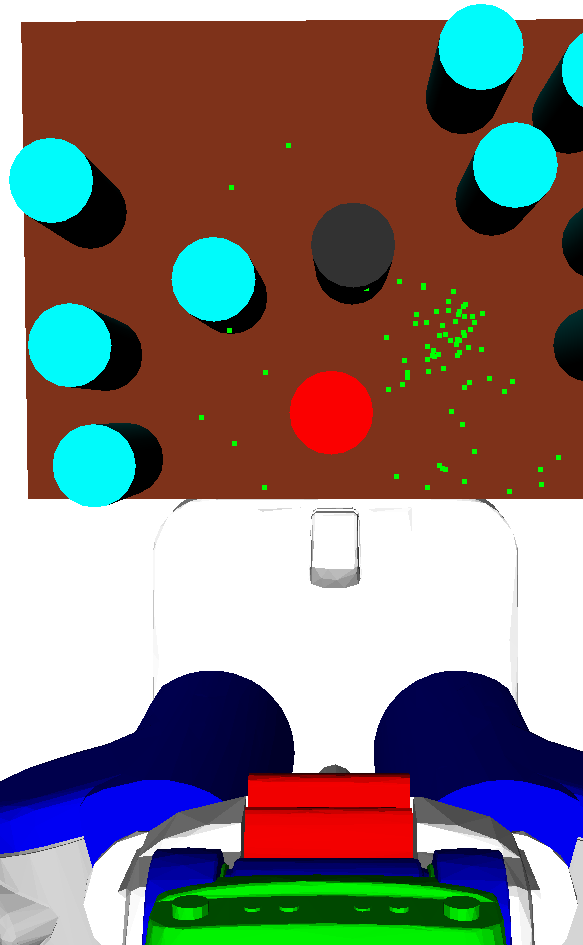
\includegraphics[scale=0.13]{images/grasp_context_1.png}
    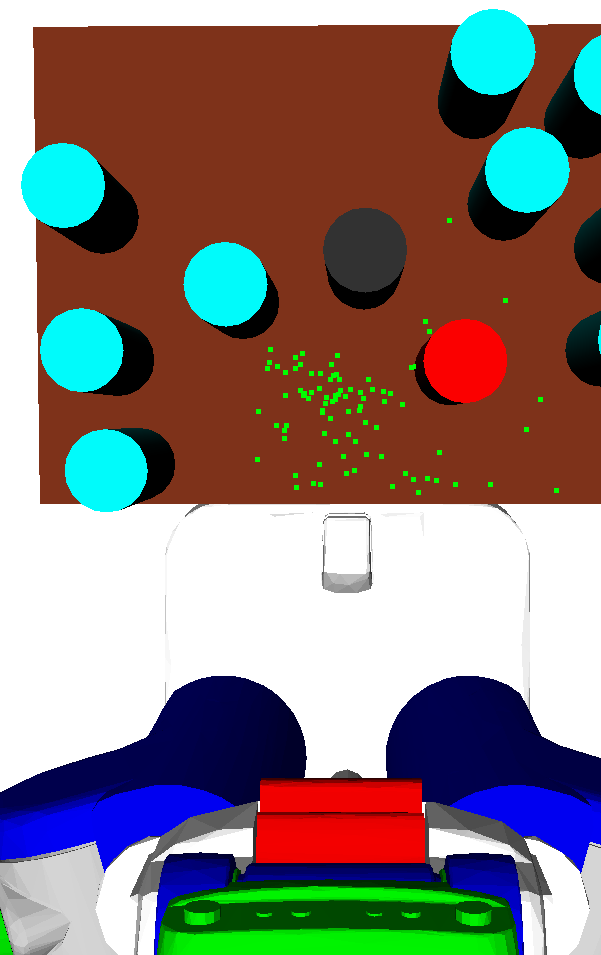
\includegraphics[scale=0.13]{images/grasp_context_2.png}
    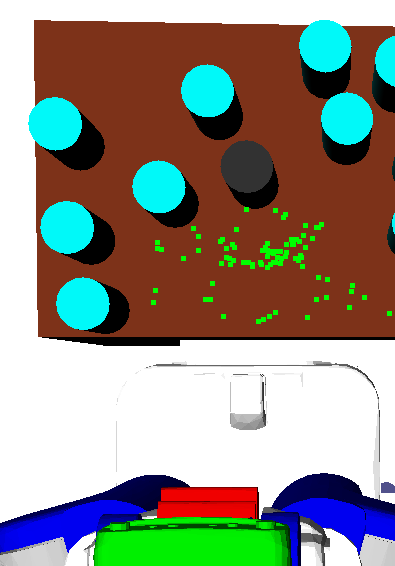
\includegraphics[scale=0.13]{images/grasp_context_3.png}
  \caption{\small{The learned left arm grasping (green) distribution
      for the black can adapts as a single potential obstruction (red) is
      moved.}}
  \label{fig:context}
\end{figure}

The results demonstrate significant improvements in performance when
compared to the baseline systems for success rate. When backtracking
search succeeds, it does so quickly, so it has a faster average
refinement time on the successes. \figref{fig:cover} shows learned
base motion and pickup distributions. \figref{fig:context} shows how
the learned distribution shifts based on the geometric context.

\subsection{Dinner Domain}
We run one set of experiments, using 4 bowls. The robot must
move the bowls from their initial locations on one table to target
locations on the other. We assign a cost to base motion in the
environment, so the robot is encouraged to use the provided tray, onto
which bowls can be stacked.  This domain has 5 types of continuous
references: base poses, object grasping poses, object putdown poses,
tray pickup poses, and tray putdown poses.

Our curriculum learning system first trains base poses and tray pickup
and putdown poses for 20 iterations, then object grasping and putdown
poses for 20 iterations. We fix $H = 100$ and $\epsilon = 10$.

The results demonstrate comparable performance to the baseline
systems. The reason is that hand-coding the sample space works well in
this domain. For example, the optimal robot base pose from which to
pick up the tray is directly in front of it, which is quickly sampled
in the baseline systems. Additionally, the lack of long-term
dependencies in the plan means that backtracking search finds a valid
refinement quickly. The fact that our system performs comparably with
the baselines shows that our learning algorithm can recover good
hand-coded distributions.  \figref{fig:cover} shows learned tray
pickup poses after all 20 iterations.

\subsection{Frying Domain}
We run two sets of experiments, using 2 and 4 frying pans. The robot
must stack the frying pans in order of decreasing radius into a narrow
shelf. To be successful, it must grasp the frying pans at the handle,
so that the handle sticks out after the pan is placed in the
shelf. This domain has 3 types of continuous references: base poses,
pan grasping poses, and pan putdown poses. 

We did not need curriculum learning. We fix $N = 30$, $H = 100$, and
$\epsilon = 5$. {\sc sfrcra-14} did not have a frying domain, so we
use the following hand-coded distribution for picking up the pans: 4
grasping poses in the cardinal directions around the lip of the pan,
and 4 equidistant along the handle.

The results demonstrate significantly higher success rate versus the
baseline systems. Similar to the can domain, when backtracking ``gets lucky'' and
picks grasping poses along the handle early in the search, it succeeds quickly, leading
to a faster average refinement time on the successes.
\figref{fig:cover} shows learned frying pan grasping poses
after all 30 iterations. Our system learned to prefer picking up the
pan at its handle to fit it into the shelf, which is not shown.






